%  LaTeX support: latex@mdpi.com
%  For support, please attach all files needed for compiling as well as the log file, and specify your operating system, LaTeX version, and LaTeX editor.

%=================================================================
% pandoc conditionals added to preserve backwards compatibility with previous versions of rticles

\documentclass[Universitat de
València,article,submit,moreauthors,pdftex]{Definitions/mdpi}


%% Some pieces required from the pandoc template
\setlist[itemize]{leftmargin=*,labelsep=5.8mm}
\setlist[enumerate]{leftmargin=*,labelsep=4.9mm}


%--------------------
% Class Options:
%--------------------

%---------
% article
%---------
% The default type of manuscript is "article", but can be replaced by:
% abstract, addendum, article, book, bookreview, briefreport, casereport, comment, commentary, communication, conferenceproceedings, correction, conferencereport, entry, expressionofconcern, extendedabstract, datadescriptor, editorial, essay, erratum, hypothesis, interestingimage, obituary, opinion, projectreport, reply, retraction, review, perspective, protocol, shortnote, studyprotocol, systematicreview, supfile, technicalnote, viewpoint, guidelines, registeredreport, tutorial
% supfile = supplementary materials

%----------
% submit
%----------
% The class option "submit" will be changed to "accept" by the Editorial Office when the paper is accepted. This will only make changes to the frontpage (e.g., the logo of the journal will get visible), the headings, and the copyright information. Also, line numbering will be removed. Journal info and pagination for accepted papers will also be assigned by the Editorial Office.

%------------------
% moreauthors
%------------------
% If there is only one author the class option oneauthor should be used. Otherwise use the class option moreauthors.

%---------
% pdftex
%---------
% The option pdftex is for use with pdfLaTeX. Remove "pdftex" for (1) compiling with LaTeX & dvi2pdf (if eps figures are used) or for (2) compiling with XeLaTeX.

%=================================================================
% MDPI internal commands - do not modify
\firstpage{1}
\makeatletter
\setcounter{page}{\@firstpage}
\makeatother
\pubvolume{1}
\issuenum{1}
\articlenumber{0}
\pubyear{2023}
\copyrightyear{2023}
%\externaleditor{Academic Editor: Firstname Lastname}
\datereceived{ }
\daterevised{ } % Comment out if no revised date
\dateaccepted{ }
\datepublished{ }
%\datecorrected{} % For corrected papers: "Corrected: XXX" date in the original paper.
%\dateretracted{} % For corrected papers: "Retracted: XXX" date in the original paper.
\hreflink{https://doi.org/} % If needed use \linebreak
%\doinum{}
%\pdfoutput=1 % Uncommented for upload to arXiv.org

%=================================================================
% Add packages and commands here. The following packages are loaded in our class file: fontenc, inputenc, calc, indentfirst, fancyhdr, graphicx, epstopdf, lastpage, ifthen, float, amsmath, amssymb, lineno, setspace, enumitem, mathpazo, booktabs, titlesec, etoolbox, tabto, xcolor, colortbl, soul, multirow, microtype, tikz, totcount, changepage, attrib, upgreek, array, tabularx, pbox, ragged2e, tocloft, marginnote, marginfix, enotez, amsthm, natbib, hyperref, cleveref, scrextend, url, geometry, newfloat, caption, draftwatermark, seqsplit
% cleveref: load \crefname definitions after \begin{document}

%=================================================================
% Please use the following mathematics environments: Theorem, Lemma, Corollary, Proposition, Characterization, Property, Problem, Example, ExamplesandDefinitions, Hypothesis, Remark, Definition, Notation, Assumption
%% For proofs, please use the proof environment (the amsthm package is loaded by the MDPI class).

%=================================================================
% Full title of the paper (Capitalized)
\Title{Análisis del mercado laboral en España}

% MDPI internal command: Title for citation in the left column
\TitleCitation{Análisis del mercado laboral en España}

% Author Orchid ID: enter ID or remove command
%\newcommand{\orcidauthorA}{0000-0000-0000-000X} % Add \orcidA{} behind the author's name
%\newcommand{\orcidauthorB}{0000-0000-0000-000X} % Add \orcidB{} behind the author's name


% Authors, for the paper (add full first names)
\Author{Catret Ruber, Pablo$^{1,2}$, Palazón Caballero, José
Miguel$^{1,3}$, Rosique Martínez, Marcos$^{1,4}$}


%\longauthorlist{yes}


% MDPI internal command: Authors, for metadata in PDF
\AuthorNames{Catret Ruber, Pablo, Palazón Caballero, José
Miguel, Rosique Martínez, Marcos}

% MDPI internal command: Authors, for citation in the left column
%\AuthorCitation{Lastname, F.; Lastname, F.; Lastname, F.}
% If this is a Chicago style journal: Lastname, Firstname, Firstname Lastname, and Firstname Lastname.
\AuthorCitation{Catret Ruber, P.; Palazón Caballero, J.M.; Rosique
Martínez, M.}

% Affiliations / Addresses (Add [1] after \address if there is only one affiliation.)
\address{%
$^{1}$ \quad Universitat de València - Escola Tècnica Superior
d'Enginyeria (ETSE) Avinguda de l'Universitat, 46100 Burjassot,
Valencia.; \\
$^{2}$ \quad Máster Universitario en Ciencia de
Datos; \href{mailto:carupa@alumni.uv.es}{\nolinkurl{carupa@alumni.uv.es}}\\
$^{3}$ \quad Máster Universitario en Ciencia de
Datos; \href{mailto:jomipaca@alumni.uv.es}{\nolinkurl{jomipaca@alumni.uv.es}}\\
$^{4}$ \quad Máster Universitario en Ciencia de
Datos; \href{mailto:rosique3@alumni.uv.es}{\nolinkurl{rosique3@alumni.uv.es}}\\
}

% Contact information of the corresponding author
\corres{Correspondence: \href{mailto:etse@uv.es}{\nolinkurl{etse@uv.es}};
Tel.: +34-963-54-3211.}

% Current address and/or shared authorship








% The commands \thirdnote{} till \eighthnote{} are available for further notes

% Simple summary

%\conference{} % An extended version of a conference paper

% Abstract (Do not insert blank lines, i.e. \\)
\abstract{Este trabajo aborda el análisis exploratorio del mercado
laboral en España como parte de la asignatura de Análisis Exploratorio
de Datos. Utiliza datos de la Encuesta de Población Activa (EPA) y la
Clasificación Nacional de Actividades Económicas (CNAE-2009), abarcando
el período entre 2002 y 2024. En el estudio se realizan técnicas de
ciencia de datos para limpiar y analizar información sobre tasas de
empleo, actividad y ocupación, desglosadas por género, grupos de edad,
regiones y sectores económicos. Se emplearon herramientas de tratamiento
y transformación de datos para unificar conjuntos, corregir valores
faltantes y estandarizar formatos, incluyendo la normalización de fechas
y la imputación de datos ausentes. Además, se integraron métricas como
tasas de actividad, empleo y desempleo, calculadas mediante fórmulas
específicas para identificar patrones y tendencias en el tiempo. Los
métodos incluyen visualizaciones gráficas para representar dinámicas
temporales y regionales, cálculos de variación entre periodos para
detectar cambios significativos y técnicas de clusterización para
analizar de manera segmentada la evolución del mercado laboral en
distintos grupos. El análisis revela el impacto de eventos como la
crisis de 2008 y la pandemia de COVID-19 en el mercado laboral,
destacando desigualdades estructurales y patrones sectoriales.}


% Keywords
\keyword{Mercado laboral; Tasa; Clustering; Pandemia COVID-19; Análisis
exploratorio de datos}

% The fields PACS, MSC, and JEL may be left empty or commented out if not applicable
%\PACS{J0101}
%\MSC{}
%\JEL{}

%%%%%%%%%%%%%%%%%%%%%%%%%%%%%%%%%%%%%%%%%%
% Only for the journal Diversity
%\LSID{\url{http://}}

%%%%%%%%%%%%%%%%%%%%%%%%%%%%%%%%%%%%%%%%%%
% Only for the journal Applied Sciences

%%%%%%%%%%%%%%%%%%%%%%%%%%%%%%%%%%%%%%%%%%

%%%%%%%%%%%%%%%%%%%%%%%%%%%%%%%%%%%%%%%%%%
% Only for the journal Data



%%%%%%%%%%%%%%%%%%%%%%%%%%%%%%%%%%%%%%%%%%
% Only for the journal Toxins


%%%%%%%%%%%%%%%%%%%%%%%%%%%%%%%%%%%%%%%%%%
% Only for the journal Encyclopedia


%%%%%%%%%%%%%%%%%%%%%%%%%%%%%%%%%%%%%%%%%%
% Only for the journal Advances in Respiratory Medicine
%\addhighlights{yes}
%\renewcommand{\addhighlights}{%

%\noindent This is an obligatory section in “Advances in Respiratory Medicine”, whose goal is to increase the discoverability and readability of the article via search engines and other scholars. Highlights should not be a copy of the abstract, but a simple text allowing the reader to quickly and simplified find out what the article is about and what can be cited from it. Each of these parts should be devoted up to 2~bullet points.\vspace{3pt}\\
%\textbf{What are the main findings?}
% \begin{itemize}[labelsep=2.5mm,topsep=-3pt]
% \item First bullet.
% \item Second bullet.
% \end{itemize}\vspace{3pt}
%\textbf{What is the implication of the main finding?}
% \begin{itemize}[labelsep=2.5mm,topsep=-3pt]
% \item First bullet.
% \item Second bullet.
% \end{itemize}
%}


%%%%%%%%%%%%%%%%%%%%%%%%%%%%%%%%%%%%%%%%%%


% tightlist command for lists without linebreak
\providecommand{\tightlist}{%
  \setlength{\itemsep}{0pt}\setlength{\parskip}{0pt}}

% From pandoc table feature
\usepackage{longtable,booktabs,array}
\usepackage{calc} % for calculating minipage widths
% Correct order of tables after \paragraph or \subparagraph
\usepackage{etoolbox}
\makeatletter
\patchcmd\longtable{\par}{\if@noskipsec\mbox{}\fi\par}{}{}
\makeatother
% Allow footnotes in longtable head/foot
\IfFileExists{footnotehyper.sty}{\usepackage{footnotehyper}}{\usepackage{footnote}}
\makesavenoteenv{longtable}


\usepackage{longtable}
\usepackage{booktabs}
\usepackage{array}
\usepackage{multirow}
\usepackage{wrapfig}
\usepackage{float}
\usepackage{colortbl}
\usepackage{pdflscape}
\usepackage{tabu}
\usepackage{threeparttable}
\usepackage{threeparttablex}
\usepackage[normalem]{ulem}
\usepackage{makecell}
\usepackage{xcolor}

\begin{document}



%%%%%%%%%%%%%%%%%%%%%%%%%%%%%%%%%%%%%%%%%%

\section{Introducción}\label{introducciuxf3n}

El mercado laboral en España es un sistema complejo y dinámico que
refleja las interacciones entre diversos factores económicos, sociales y
demográficos. Este trabajo de análisis exploratorio de datos combina dos
pilares fundamentales para entender las dinámicas laborales: la Encuesta
de Población Activa (EPA) y la Clasificación Nacional de Actividades
Económicas (CNAE-2009). A través de estas fuentes, se busca ofrecer una
visión integral de las tasas de empleo, actividad y ocupación,
desglosadas por género, grupo de edad y comunidad autónoma, así como por
ramas de actividad económica.

La EPA, realizada trimestralmente por el Instituto Nacional de
Estadística (INE), proporciona información detallada sobre la
participación laboral de la población, permitiendo analizar las
diferencias en el acceso al empleo según el género, la edad y el
territorio. En esta parte del estudio, se examinan las tasas del mercado
laboral en las distintas comunidades autónomas y cómo estas se ven
influenciadas por eventos como la crisis financiera de 2008 o la
pandemia de COVID-19. Además, se busca identificar desigualdades
estructurales y dinámicas regionales que puedan servir como base para
estudios más específicos o el diseño de políticas públicas.

Por otro lado, la CNAE-2009 aporta un marco estándar para clasificar las
actividades económicas en las que se desempeñan los trabajadores,
permitiendo analizar cómo se distribuye la fuerza laboral entre
diferentes sectores. Este enfoque complementario permite explorar no
solo el ``dónde'' y ``quién'' trabaja, sino también el ``en qué''
trabaja la población, revelando patrones de especialización sectorial y
el impacto de la transformación económica a lo largo de los años.

La combinación de ambas perspectivas ---la distribución demográfica y
regional desde la EPA y la estructura sectorial desde la CNAE--- permite
abordar preguntas clave sobre el mercado laboral, tales como:

\begin{itemize}
\tightlist
\item
  ¿Cómo varía la participación laboral entre comunidades autónomas?
\item
  ¿Cómo varía la participación laboral entre grupos de edad?
\item
  ¿Qué sectores han experimentado los mayores cambios tras eventos
  históricos como la crisis de 2008 o la pandemia de COVID-19?
\end{itemize}

Este análisis exploratorio busca no solo describir el estado actual del
mercado laboral en España, sino también identificar tendencias,
desigualdades y oportunidades de mejora. El objetivo final es
proporcionar una base sólida para futuros estudios y contribuir al
diseño de estrategias efectivas en el ámbito económico, social y
político.

\section{Importación y tratamiento de
datos}\label{importaciuxf3n-y-tratamiento-de-datos}

En primer lugar, se han descargado los datos directamente desde la base
de datos abierta INE Base. Estos datos se presentan en un formato de
csv, separado por el carácter `;', y con el uso de marca de decimales
española `,'.

\subsection{\texorpdfstring{\textbf{Encuesta de Población Activa
(EPA)}}{Encuesta de Población Activa (EPA)}}\label{encuesta-de-poblaciuxf3n-activa-epa}

Como se ha mencionado anteriormente en la introducción, la EPA es
realizada trimestralmente por el Instituto Nacional de Estadística, por
lo que se han extraído cinco datasets de su base de datos: población
total, activa, inactiva, ocupada y parada.

Cabe destacar que estos datasets están desglosados por comunidad y
ciudad autónoma, sexo y grupo de edad, con las tres columnas expresadas
en ``miles de personas'' como unidad. El periodo de los datos figura
desde el primer trismestre de 2002 hasta el tercer trimestre de 2024.

Al tratarse de un análisis del mercado laboral eliminaremos al grupo de
población menor a 16 años pues no tienen edad suficiente para trabajar.
Notamos que en el dataset Población hay una columna que solo contiene la
cadena ``Total Nacional'', por lo que la eliminamos. Además, en la
columna ``Comunidades y Ciudades Autónomas'' hay valores faltantes que
coinciden con las filas del propio Total Nacional, de modo que los
completamos con dicha cadena.

Notamos que para el conjunto de datos de población total en edad de
trabajar y población inactiva hay un intervalo de edad más que para el
resto de datasets: se divide ``55 y más años'' en los grupos ``De 55 a
64 años'' y ``65 y más años''. Dado que buscamos obtener un dataset
único y compacto uniremos ambos grupos de edad como en el resto de
datasets. Una vez normalizada la estructura de los datasets podemos
unificarlos.

Otra circunstancia a corregir que los datos de la columna ``Periodo''
son cadenas; para solucionarlo, definimos y empleamos la función
``SacarFechas'' para transformarlos a tipo Date. Una vez corregido,
comprobaremos si existen datos faltantes en nuestro dataset.

\begin{longtable}[]{@{}lr@{}}
\caption{Frecuencias de datos faltantes en el conjunto de datos
EPA}\tabularnewline
\toprule\noalign{}
Variable & Valores faltantes \\
\midrule\noalign{}
\endfirsthead
\toprule\noalign{}
Variable & Valores faltantes \\
\midrule\noalign{}
\endhead
\bottomrule\noalign{}
\endlastfoot
Sexo & 0 \\
Comunidades y Ciudades Autónomas & 0 \\
Edad & 0 \\
Periodo & 0 \\
Población en edad de trabajar & 0 \\
Activos & 43 \\
Inactivos & 0 \\
Ocupados & 277 \\
Parados & 272 \\
\end{longtable}

Existe únicamente un porcentaje muy bajo de valores faltantes entre las
columnas ``Activos'', ``Ocupados'' y ``Parados''. Veamos un ejemplo de
estos casos.

\begin{longtable}[]{@{}lr@{}}
\caption{Frecuencias de datos faltantes por Comunidad Autónoma en el
conjunto de datos EPA}\tabularnewline
\toprule\noalign{}
Comunidad & Valores faltantes \\
\midrule\noalign{}
\endfirsthead
\toprule\noalign{}
Comunidad & Valores faltantes \\
\midrule\noalign{}
\endhead
\bottomrule\noalign{}
\endlastfoot
02 Aragón & 1 \\
03 Asturias, Principado de & 12 \\
04 Balears, Illes & 1 \\
05 Canarias & 5 \\
06 Cantabria & 18 \\
11 Extremadura & 6 \\
15 Navarra, Comunidad Foral de & 12 \\
16 País Vasco & 3 \\
17 Rioja, La & 19 \\
18 Ceuta & 182 \\
19 Melilla & 247 \\
\end{longtable}

\begin{longtable}[]{@{}lr@{}}
\caption{Frecuencias de datos faltantes por edad en el conjunto de datos
EPA}\tabularnewline
\toprule\noalign{}
Grupo de edad & Valores faltantes \\
\midrule\noalign{}
\endfirsthead
\toprule\noalign{}
Grupo de edad & Valores faltantes \\
\midrule\noalign{}
\endhead
\bottomrule\noalign{}
\endlastfoot
55 y más años & 101 \\
De 16 a 19 años & 345 \\
De 20 a 24 años & 18 \\
De 25 a 34 años & 1 \\
De 35 a 44 años & 13 \\
De 45 a 54 años & 27 \\
Total & 1 \\
\end{longtable}

Los datos se concentran en Comunidades y Ciudades Autónomas con
proporcionalmente poca población y en rangos de edades donde es poco
habitual estar ocupado (ya que para que se cumpla dicha condición se
debe estar buscando activamente trabajo). De hecho, el único valor que
podría resultar extraño es que exista un valor faltante para un Total de
edades, pero al comprobar la localización y fecha notamos que es
razonable.

\begin{longtable}[]{@{}lll@{}}
\caption{Valor faltante en el total de edades en el conjunto de datos
EPA}\tabularnewline
\toprule\noalign{}
Sexo & Comunidades y Ciudades Autónomas & Periodo \\
\midrule\noalign{}
\endfirsthead
\toprule\noalign{}
Sexo & Comunidades y Ciudades Autónomas & Periodo \\
\midrule\noalign{}
\endhead
\bottomrule\noalign{}
\endlastfoot
Hombres & 19 Melilla & 2002-06-01 \\
\end{longtable}

Dicho patrón parece reflejar que muy poca población de esas
características se encontraba parada; por tanto, sustituiremos los
valores faltantes del dataset por ceros.

\subsection{\texorpdfstring{\textbf{Clasificación Nacional de
Actividades Económicas
(CNAE-2009)}}{Clasificación Nacional de Actividades Económicas (CNAE-2009)}}\label{clasificaciuxf3n-nacional-de-actividades-econuxf3micas-cnae-2009}

Este dataset divide los datos según rama de actividad, sexo y fecha en
el periodo comprendido entre el primer trimestre de 2008 y el tercer
trimestre de 2024, usando las mismas unidades que en el resto de
datasets. No obstante, en este caso podemos encontrar los datos
segmentado en dos subconjuntos principales:

\begin{itemize}
\item
  Porcentajes (``Total\_abs''): Representan la proporción de ocupación
  de cada rama de actividad con respecto al total del sexo
  correspondiente.
\item
  Valores absolutos (``Total\_porc''): Proporcionan el número total de
  empleados en cada rama.
\end{itemize}

Esta separación permite analizar tanto las tendencias globales (valores
absolutos) como la estructura relativa de los sectores (porcentajes).

Nos encontramos de nuevo con el problema del formato de las fechas, por
lo que volveremos a aplicar la función SacarFechas. Además, para
diferenciar entre cada tipo de dato (valor absoluto y porcentaje) vamos
a extraerlos en dos datasets para posteriormente realizar un join,
esencialmente como si se realizara un pivote. Una vez hemos unificado la
tabla es recomendable realizar un análisis de datos faltantes.

\begin{longtable}[]{@{}lr@{}}
\caption{Frecuencias de datos faltantes en el conjunto de datos
CNAE}\tabularnewline
\toprule\noalign{}
Variable & Valores faltantes \\
\midrule\noalign{}
\endfirsthead
\toprule\noalign{}
Variable & Valores faltantes \\
\midrule\noalign{}
\endhead
\bottomrule\noalign{}
\endlastfoot
Rama.de.actividad.CNAE.2009 & 0 \\
Sexo & 0 \\
Periodo & 0 \\
Total\_abs & 313 \\
Total\_porc & 313 \\
\end{longtable}

Observamos que para un pequeño subconjunto de filas no existen cifras
totales. Veamos si siguen algún patrón.

\begin{longtable}[]{@{}l@{}}
\caption{Primeras cuatro actividades con valores faltantes en
Total\_abs}\tabularnewline
\toprule\noalign{}
Rama de actividad \\
\midrule\noalign{}
\endfirsthead
\toprule\noalign{}
Rama de actividad \\
\midrule\noalign{}
\endhead
\bottomrule\noalign{}
\endlastfoot
05 Extracción de antracita, hulla y lignito \\
06 Extracción de crudo de petróleo y gas natural \\
07 Extracción de minerales metálicos \\
09 Actividades de apoyo a las industrias extractivas \\
\end{longtable}

Notamos que los valores faltantes se encuentran en ramas de actividades
poco comunes relacionadas con la industria pesada, por lo que dichos NA
reflejarán que muy poca población se dedica a ello, probablemente menos
del mínimo registrable; en consecuencia sustituiremos dichos valores por
ceros.

Por último, añadiremos una columna que calcula la variación entre un
periodo y el siguiente, lo que permitirá identificar momentos de cambio
significativo en el mercado laboral, detectando tendencias positivas o
negativas a lo largo del tiempo. Esto también permitirá ver de manera
rápida la estacionalidad de la ocupación, sobre todo en ciertas ramas de
actividad. Es importante mencionar que realizar las diferencias entre un
periodo y el siguiente genera NAs para el primer periodo de cada rama,
por lo que sustituiremos estos valores faltantes por ceros.

\section{Representación y análisis de
datos}\label{representaciuxf3n-y-anuxe1lisis-de-datos}

Una vez preparados, los datos se visualizan a través de gráficos y tasas
que permiten interpretar patrones, tendencias y distribuciones de manera
más clara y directa.

\subsection{\texorpdfstring{\textbf{Encuesta de Población Activa
(EPA)}}{Encuesta de Población Activa (EPA)}}\label{encuesta-de-poblaciuxf3n-activa-epa-1}

Las tasas del mercado de trabajo, como la de actividad, empleo y
ocupación, son fundamentales para este análisis porque permiten comparar
de forma clara y estandarizada las dinámicas laborales entre comunidades
autónomas y grupos poblacionales. Estas métricas facilitan el estudio de
tendencias temporales y desigualdades estructurales, como las brechas de
género o regionales, que no serían evidentes al observar valores
absolutos. Además, su uso es clave para identificar áreas críticas y
evaluar el impacto de eventos económicos, como la crisis de 2008 o la
pandemia de COVID-19, en la participación laboral de la población.

Por ello, las siguientes tasas quedan incorporadas dentro del dataset
anteriormente mencionado:

\begin{itemize}
\item
  Tasa de Actividad (TA) =
  \(\frac{\text{Activos}}{\text{Población} \geq 16}\cdot100\)
\item
  Tasa de Inactividad (TI) =
  \(\frac{\text{Inactivos}}{\text{Población} \geq 16}\cdot100 = 1 - TA\)
\item
  Tasa de Ocupación (TO) =
  \(\frac{\text{Ocupados}}{\text{Población} \geq 16}\cdot100\)
\item
  Tasa de Empleo (TE) =
  \(\frac{\text{Ocupados}}{\text{Activos}}\cdot100\)
\item
  Tasa de Desempleo (TD) =
  \(\frac{\text{Parados}}{\text{Activos}}\cdot100 = 1 - TE\)
\end{itemize}

\begin{figure}[h]

{\centering 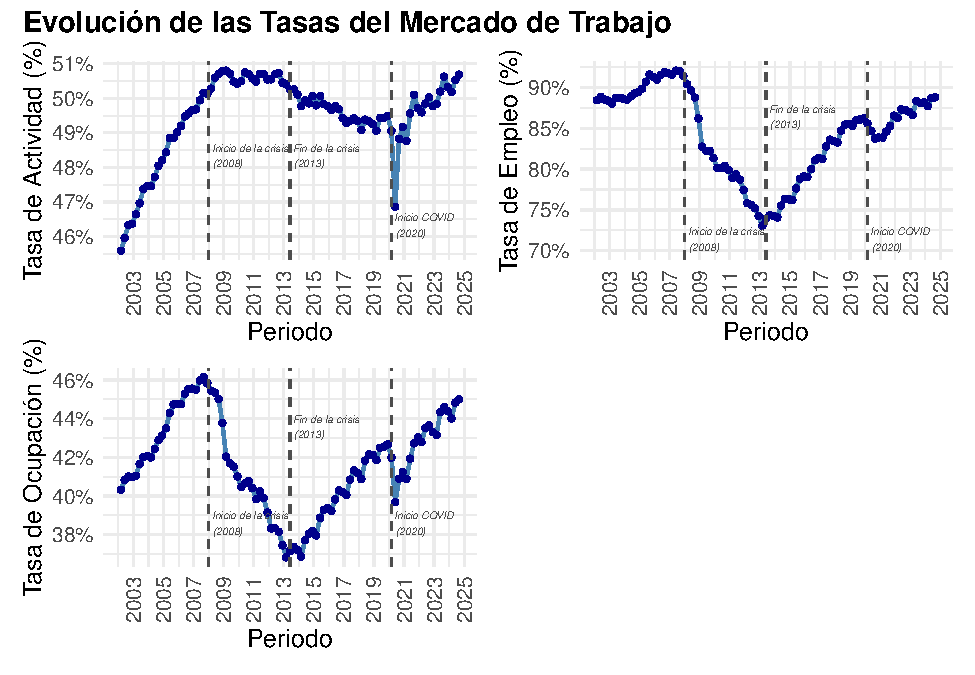
\includegraphics[width=1\linewidth]{ProyectoAED2024_files/figure-latex/unnamed-chunk-26-1} 

}

\caption{Evolución del mercado de trabajo en España}\label{fig:unnamed-chunk-26}
\end{figure}

La Figura 1 muestra la evolución de la tasa de actividad, empleo y
ocupación en España desde 2002 hasta la actualidad, reflejando cambios
asociados a eventos económicos y sociales. Entre 2002 y 2008, todas las
tasas crecieron sostenidamente gracias a la bonanza económica, mientras
que la crisis de 2008 provocó una fuerte caída en las tasas de empleo y
ocupación, aunque la tasa de actividad se mantuvo estable hasta 2013. En
ese periodo, el empleo cayó a niveles del 75\%, evidenciando un
desempleo superior al 25\%.

Desde 2013, con signos de recuperación económica, las tasas de empleo y
ocupación comenzaron a mejorar progresivamente, mientras que la tasa de
actividad decreció ligeramente debido a factores como la reducción del
abandono escolar. La pandemia de COVID-19 en 2020 generó caídas abruptas
en todas las tasas, especialmente en la ocupación, aunque a partir de
2021 se observa una recuperación marcada por la reincorporación laboral
y el dinamismo de sectores clave como el turismo y los servicios
digitales.

\begin{figure}[h]

{\centering 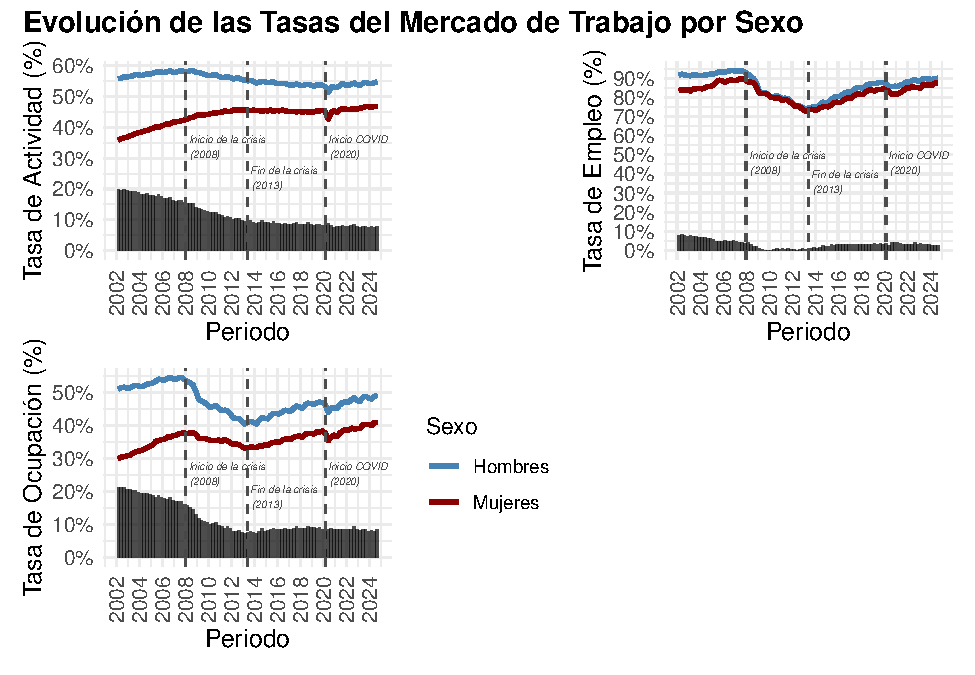
\includegraphics[width=1\linewidth]{ProyectoAED2024_files/figure-latex/unnamed-chunk-28-1} 

}

\caption{Evolución del mercado de trabajo por género en España}\label{fig:unnamed-chunk-28}
\end{figure}

En cambio, la Figura 2 muestra la evolución de las tasas de actividad,
empleo y ocupación por género, evidenciando desigualdades y avances
hacia la igualdad. La tasa de actividad masculina, aunque más alta,
disminuyó entre 2008 y 2020, mientras que la femenina creció
sostenidamente desde 2002, reduciendo la brecha de género del 20\% al
8\%. En la tasa de empleo, las diferencias son menores, ya que mide solo
a la población activa, mientras que en la tasa de ocupación las
disparidades son más evidentes al incluir a toda la población en edad de
trabajar.

La pandemia de 2020 generó descensos significativos en todas las tasas,
seguidos de una recuperación que refleja la resiliencia del mercado
laboral. Este análisis resalta los avances hacia la igualdad laboral,
aunque persisten desigualdades estructurales, especialmente en la
población activa y su impacto en la ocupación.\newline

\begin{figure}[h]

{\centering 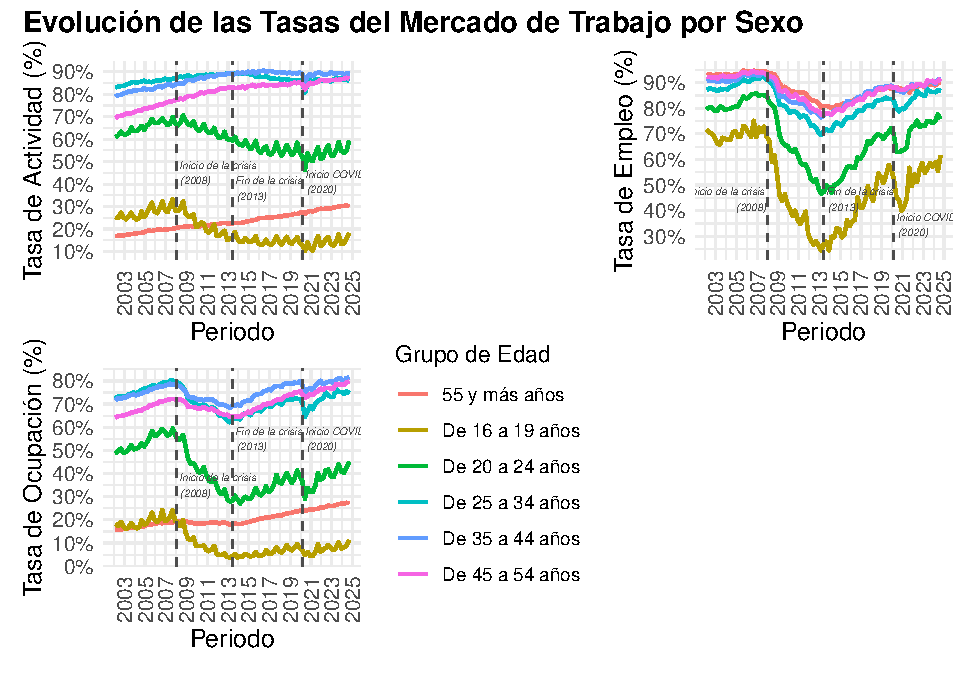
\includegraphics[width=1\linewidth]{ProyectoAED2024_files/figure-latex/unnamed-chunk-30-1} 

}

\caption{Evolución del mercado de trabajo por grupo de edad en España}\label{fig:unnamed-chunk-30}
\end{figure}

Por último, referenciando a la Figura 3 que desglosa la población por
grupos de edad, se puede observar cómo los grupos de edad han
experimentado dinámicas distintas en el mercado laboral. Los mayores de
35 a 54 años mantienen tasas de actividad superiores al 80 \%,
reflejando una integración estable. En contraste, los jóvenes de 16 a 24
años presentan tasas mucho más bajas, con un desempleo superior al 70 \%
en 2013, influido por la crisis en sectores como la construcción y el
aumento de la escolarización.

Los grupos jóvenes también exhiben estacionalidad, especialmente en
verano, cuando se incorporan al mercado laboral en sectores como la
hostelería. Por otro lado, el grupo de 55 y más años presenta tasas de
actividad y ocupación bajas debido a la jubilación, aunque esto no
afecta de igual manera a la tasa de empleo, que excluye a los inactivos
como los jubilados.

\subsubsection{\texorpdfstring{\textbf{Clusterización por Comunidades y
Ciudades
Autónomas}}{Clusterización por Comunidades y Ciudades Autónomas}}\label{clusterizaciuxf3n-por-comunidades-y-ciudades-autuxf3nomas}

En este apartado del proyecto se va a proceder a realizar un clustering
de la tasa de empleo para las distintas Comunidades y Ciudades Autónomas
de España en los siguientes años: 2007, 2013 y 2023. El principal motivo
por el cual escogemos esta tasa se debe a que se mide como el porcentaje
de personas ocupadas respecto a la población activa, es decir, las que
se encuentran activamente en el mercado laboral.

Como método de clusterización se utilizará el k-means, que organiza los
datos en grupos basados en su similitud. Este algoritmo comienza
eligiendo un número de clusters (\texttt{k}) y seleccionando centroides
iniciales al azar. Cada punto se asigna al clúster cuyo centroide está
más cercano, y luego los centroides se recalculan como el promedio de
los puntos en cada grupo. Es un proceso que se repite hasta que los
centroides dejan de cambiar o se alcanza un límite de iteraciones. Al
finalizar, las comunidades quedan agrupadas en k clusters representando
cada uno un conjunto de puntos con características similares, en este
caso CCAA.

Por otro lado, para la selección del hiperparámetro \texttt{k} se opta
por el método del codo. Este consiste en graficar la suma de cuadrados
dentro del clúster (WSS) frente a distintos valores de \texttt{k}. El
punto donde la disminución de WSS se ralentiza significativamente,
formando un ``codo'', indica el número adecuado de clusters.\newline

\begin{figure}[h]

{\centering 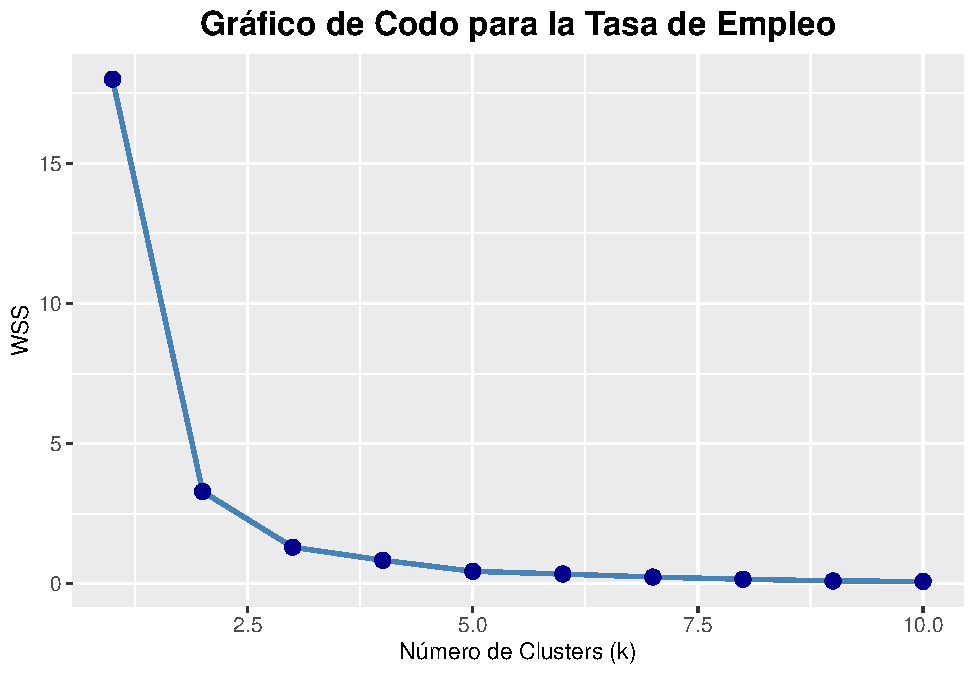
\includegraphics[width=0.4\linewidth]{ProyectoAED2024_files/figure-latex/unnamed-chunk-34-1} 

}

\caption{Gráfico de codo global para la tasa de empleo}\label{fig:unnamed-chunk-34}
\end{figure}

Observando el gráfico de la Figura 4, se puede considerar que el número
de clusters a partir del cual la WSS se ralentiza es en \texttt{k=3},
pues es en donde se forma el ``codo''.

Posteriormente, y como se ha mencionado al principio del apartado, vamos
a hacer un clustering con el objetivo de agrupar las CCAA según su tasa
de empleo en distintos periodos. Posteriormente los colores de los
clusters se representan en un mapa de España dividido por dichas
regiones para visualizar de forma clara y efectiva los patrones
espaciales. La intención de esta medida es identificar patrones
regionales y analizar las diferencias en las dinámicas del mercado
laboral a nivel territorial.\newline

\begin{figure}[h]

{\centering 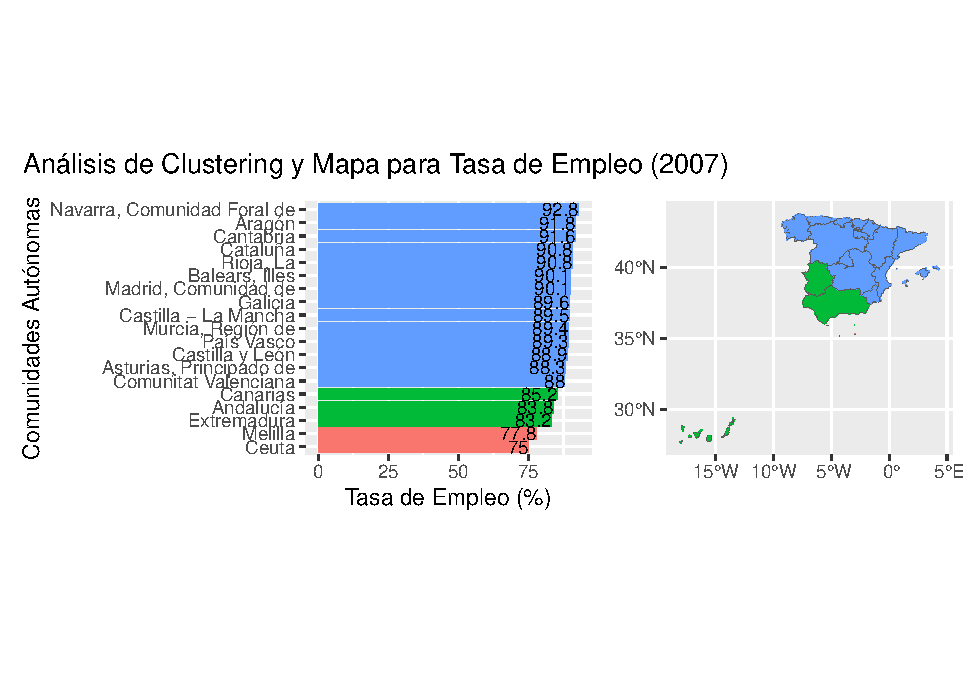
\includegraphics[width=0.9\linewidth]{ProyectoAED2024_files/figure-latex/unnamed-chunk-35-1} 

}

\caption{Clusterización regional con 3 centroides para la tasa de empleo en España en 2007}\label{fig:unnamed-chunk-35}
\end{figure}

La Figura 5 muestra el análisis de clustering de la tasa de empleo en
España en 2007. Todas las comunidades de la península a excepción de
Extremadura y Andalucía se agrupan en un clustering único debido a la
similitud en su tasa, con valores superiores al 90\% representando
mercados laborales sólidos. Ceuta y Melilla, con tasas por debajo del
80\%, pertenecen al clúster rojo, reflejando mayores desafíos laborales.
El clúster verde, con tasas entre el 80\% y el 85\%, incluye las
regiones de Extremadura, Andalucía y Canarias, que muestran estabilidad
moderada. En conjunto, la figura evidencia claras disparidades
regionales en el empleo respecto al sur del país antes de la crisis
económica.\newline

\begin{figure}[h]

{\centering 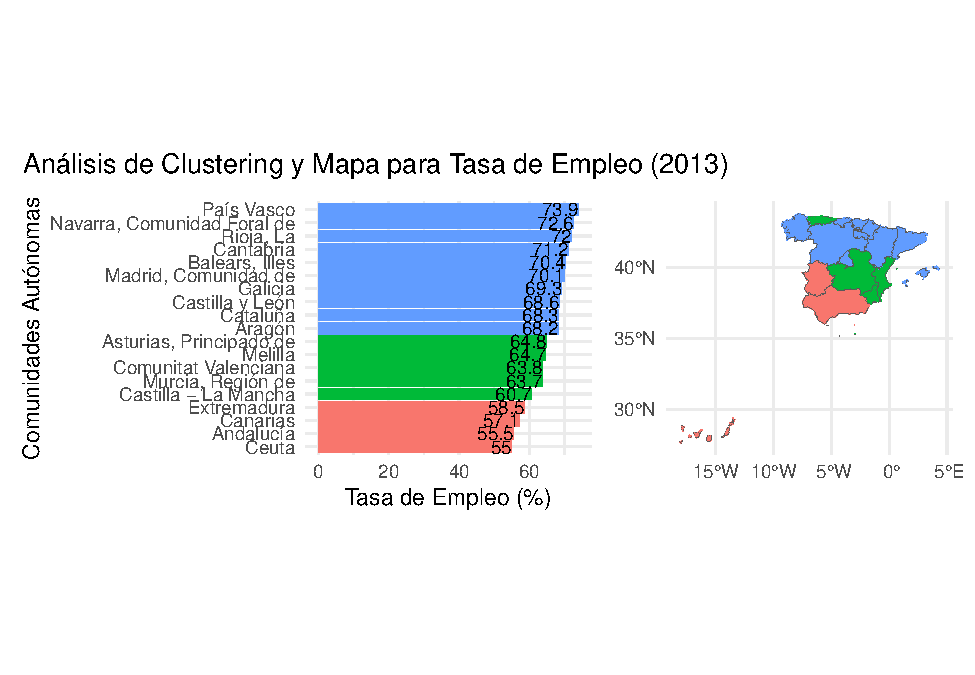
\includegraphics[width=0.9\linewidth]{ProyectoAED2024_files/figure-latex/unnamed-chunk-36-1} 

}

\caption{Clusterización regional con 3 centroides para la tasa de empleo en España en 2013}\label{fig:unnamed-chunk-36}
\end{figure}

En cambio, la Figura 6 muestra el análisis de clustering de la tasa de
empleo en España en 2013, el peor momento de la crisis económica. En
comparación con 2007, las tasas de empleo han disminuido
significativamente en todas las comunidades autónomas, reflejando el
impacto generalizado de la recesión. Mientras que en 2007 gran parte de
la península estaba agrupada en un único clúster, en 2013 se observa una
mayor dispersión. El clúster azul mantiene las tasas más altas,
superiores al 70\%, mientras que el clúster rojo refleja las más bajas,
por debajo del 60\%. Esto evidencia las desigualdades regionales
acentuadas por la crisis.\newline

\begin{figure}[h]

{\centering 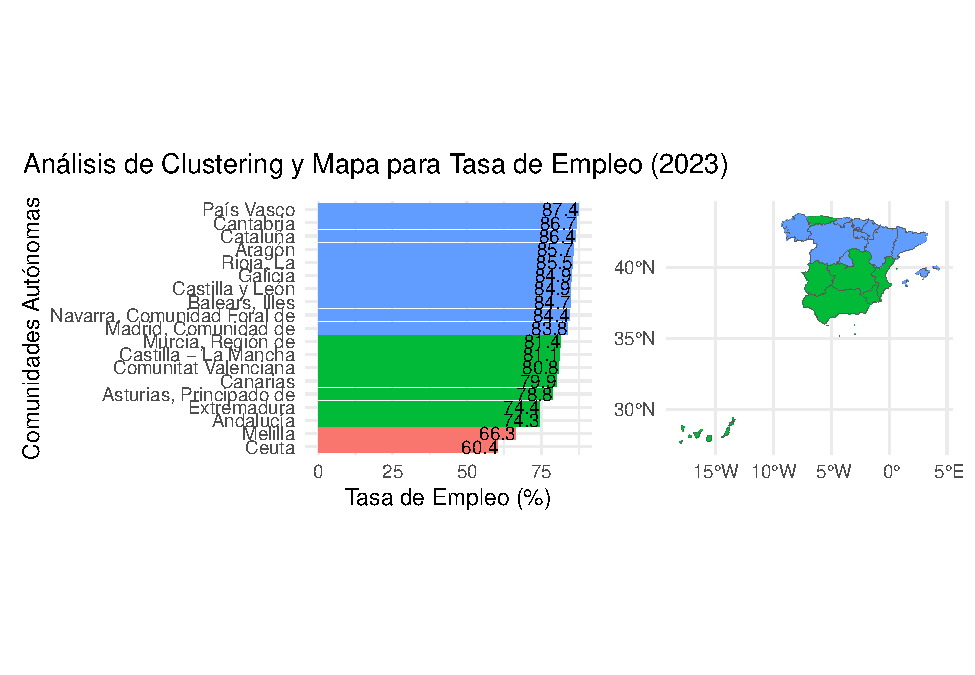
\includegraphics[width=0.9\linewidth]{ProyectoAED2024_files/figure-latex/unnamed-chunk-37-1} 

}

\caption{Clusterización regional con 3 centroides para la tasa de empleo en España en 2023}\label{fig:unnamed-chunk-37}
\end{figure}

En la actualidad, la Figura 7 muestra una recuperación general en las
tasas de empleo respecto a 2013, aunque persisten desigualdades
regionales. El clúster azul, que representa la mitad norte de España (a
excepción de Asturias), destaca con tasas superiores al 83\%, reflejando
un mercado laboral sólido en esta área. El clúster verde, que representa
la mitad sur, presenta tasas intermedias entre el 74\% y el 82\%,
reflejando una mayor estabilidad en el empleo, aunque todavía sin
alcanzar la uniformidad observada antes de la crisis. Por el contrario,
el clúster rojo, que incluye las ciudades de Ceuta y Melilla, presenta
tasas inferiores al 70\%, evidenciando desafíos laborales persistentes.

En conclusión, se evidencia una mejora general, pero con brechas
regionales significativas.

\subsection{\texorpdfstring{\textbf{Clasificación Nacional de
Actividades Económicas
(CNAE-2009)}}{Clasificación Nacional de Actividades Económicas (CNAE-2009)}}\label{clasificaciuxf3n-nacional-de-actividades-econuxf3micas-cnae-2009-1}

En primer lugar se analiza la distribución de peso de las ramas de
actividad en el total de la población empleada. Además, se busca
comparar la evolución y el cambio sufrido por la estructura laboral
española desde el primer trimestre de 2008 y el tercer trimestre de
2024. Para ello se generan treemaps para los periodos inicial (2008T1) y
final (2024T3) del análisis. Estos gráficos muestran cómo se distribuye
el empleo entre las diferentes ramas económicas según su peso relativo.

\begin{figure}

{\centering 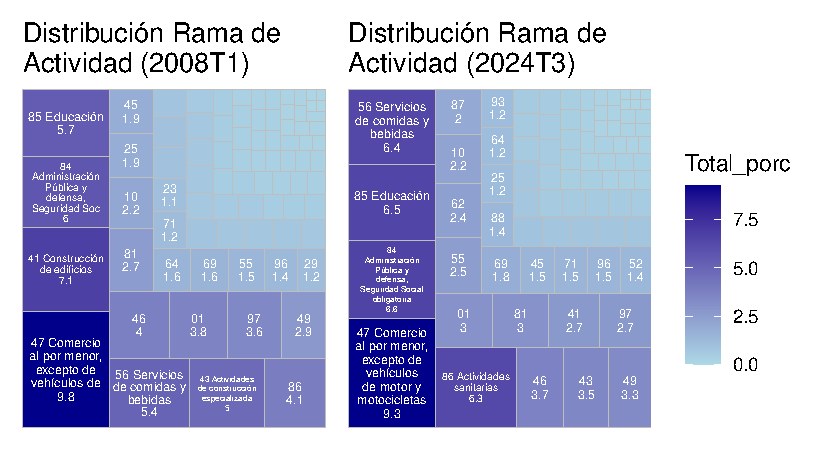
\includegraphics{ProyectoAED2024_files/figure-latex/unnamed-chunk-38-1} 

}

\caption{Distribución de las ramas de actividad en el primer trimestre de 2008 y el tercer trimestre de 2024.}\label{fig:unnamed-chunk-38}
\end{figure}

En la Figura 8 podemos observar cómo algunas ramas han ganado o perdido
relevancia en términos de empleo total a lo largo del tiempo. Por
ejemplo, sectores relacionados con la educación y la administración
pública han aumentado su proporción, mientras que ramas relacionadas con
la construcción y la industria han experimentado una marcada
disminución.

Además de realizar un análisis comparativo de cómo se distribuye por
ramas de actividad la población trabajadora, se realiza un análisis
visual de la evolución del empleo en España de manera absoluta agrupando
por sexo, en conjunto con un análisis de la evolución de la diferencia
trimestral en el empleo. Para ello se han empleado gráficos de lineas.
Estos gráficos incluyen referencias visuales a eventos históricos
relevantes, como el fin de la crisis económica de 2013 y el inicio de la
pandemia en 2020.

\begin{figure}

{\centering 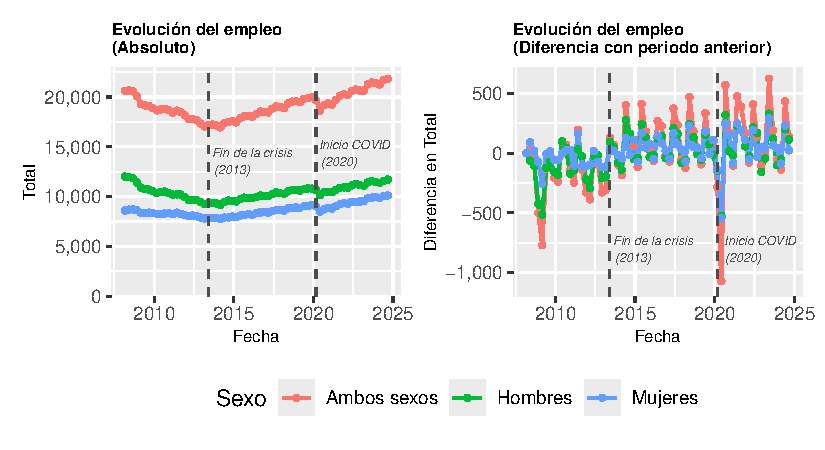
\includegraphics{ProyectoAED2024_files/figure-latex/unnamed-chunk-39-1} 

}

\caption{Evolución del empleo en España y de las diferencias ientre dos periodos consecutivos.}\label{fig:unnamed-chunk-39}
\end{figure}

En la Figura 9 destaca cómo el empleo masculino y femenino responden de
manera diferente a los shocks económicos. Por ejemplo, los hombres
experimentaron caídas más pronunciadas durante la crisis de 2008,
mientras que las mujeres mostraron una recuperación más gradual. Además,
se puede apreciar que la diferencia entre sexos se redujo en grán medida
durante la crisis de 2008, desde la cual la población masculina ha sido
incapaz de recuperar las cifras precrisis, mientras que las mujeres han
superado marcadamente dichos valores.

\subsubsection{\texorpdfstring{\textbf{Estudio de correlaciones entre
Ramas de
Actividad}}{Estudio de correlaciones entre Ramas de Actividad}}\label{estudio-de-correlaciones-entre-ramas-de-actividad}

A continuación, se realiza un estudio de las correlaciones lineales de
Pearson entre distintas ramas de actividad (en ambos sexos en conjunto).
Los datos de CNAE vienen dispuestos en dos órdenes de agrupación, unos
más generales, caracterizados por empezar por una letra en su nombre, y
otros más concretos, empezando por un número. Realizaremos el estudio
sobre los datos agrupados de forma más general, usando solo la letra
como etiqueta; el nombre completo de la rama se puede consultar en el
Apéndice.

\begin{figure}

{\centering 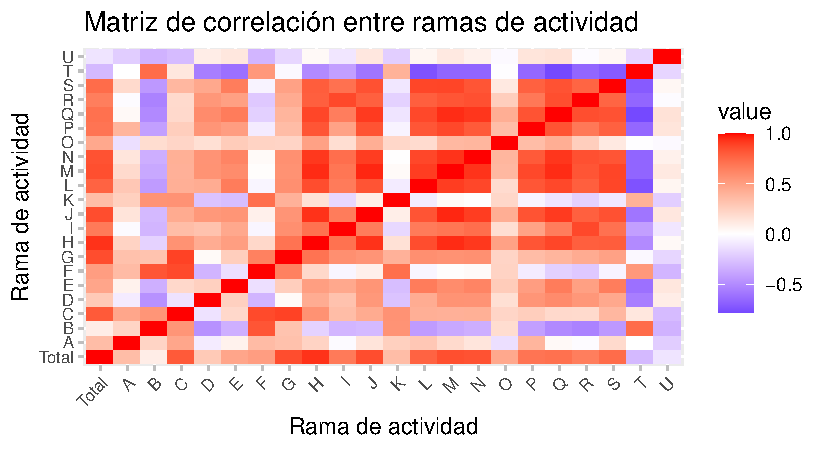
\includegraphics{ProyectoAED2024_files/figure-latex/unnamed-chunk-40-1} 

}

\caption{Matriz de correlación entre agrupaciones generales de ramas de actividad.}\label{fig:unnamed-chunk-40}
\end{figure}

En la matriz de correlación de la Figura 10 se contempla que la mayoría
de las ramas parecen estar correlacionadas positivamente, salvo aquellos
puestos relacionados con el personal doméstico e industrias extractivas
con una correlación negativa con la mayoría de las ramas, así como
aquellas relacionadas con la agricultura, ganadería, construcción,
actividades financieras entre otras que no presentan una marcada
correlación con el resto.

\subsubsection{\texorpdfstring{\textbf{Tendencias relativas a partir de
datos
normalizados}}{Tendencias relativas a partir de datos normalizados}}\label{tendencias-relativas-a-partir-de-datos-normalizados}

En este punto, se busca estudiar las tendencias relativas, eliminando la
influencia de las diferencias inciales entre ramas. Para ello, primero
se normalizan los datos dividiendo por el número inicial de trabajadores
en cada rama, y a continuación se obtiene una métrica de distancia entre
dichos datos normalizados, obteniéndose como la media de las diferencias
absolutas de las cantidades normalizadas. A partir de estas distancias,
se proyectan en dos dimensiones utilizando MDS, lo que permite
visualizar las relaciones entre ramas en función de sus patrones de
empleo a lo largo del tiempo. La proyección MDS es escogida frente a
otros métodos debido a su enfoque en conservar las distancias
establecidas.

\begin{figure}

{\centering 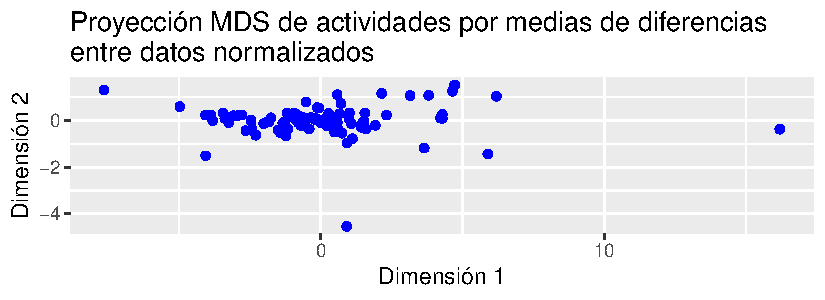
\includegraphics{ProyectoAED2024_files/figure-latex/unnamed-chunk-42-1} 

}

\caption{Proyección MDS de las distancias entre la evolución de ramas de actividad normalizadas.}\label{fig:unnamed-chunk-42}
\end{figure}

Se forman agrupaciones naturales de ramas con patrones similares en la
Figura 11. Además, se observan claramente algunos outliers, que puede
ser de gran interés analizarlos individualmente.

\begin{figure}

{\centering 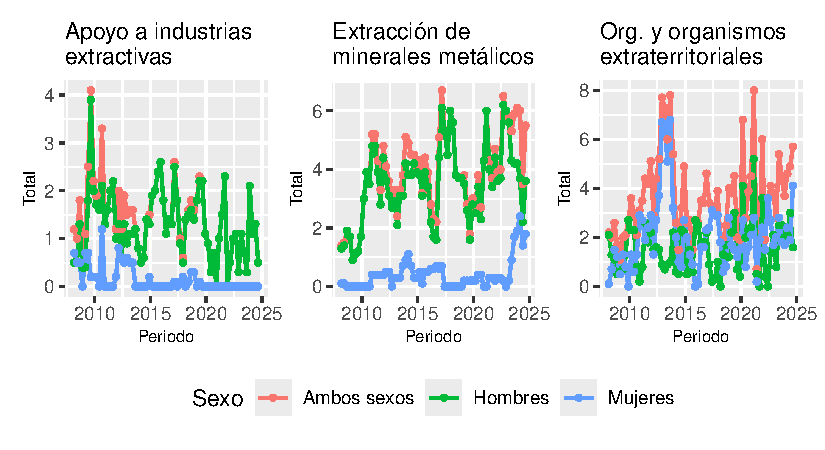
\includegraphics{ProyectoAED2024_files/figure-latex/unnamed-chunk-43-1} 

}

\caption{Evolución del empleo en posibles outliers de ramas de actividad.}\label{fig:unnamed-chunk-43}
\end{figure}

Ramas como ``Extracción de minerales metálicos'', ``Actividades de apoyo
a las industrias extractivas'' o ``Actividades de organizaciones y
organismos extraterritoriales'' se destacan en la Figura 12 por su
comportamiento atípico. Estas ramas tienen una dinámica de empleo
inusual debido a su naturaleza específica, tamaño reducido o dependencia
de factores externos como la demanda global. Observamos claramente que
son datos con mucho ruido, y por lo tanto es normal que nos apareciesen
como outliers.

\subsubsection{\texorpdfstring{\textbf{Clusterización por Ramas de
Actividad}}{Clusterización por Ramas de Actividad}}\label{clusterizaciuxf3n-por-ramas-de-actividad}

Tras observar la proyección tratamos de segmentar los datos en
agrupaciones naturales, es por ello que tratamos de hacer un clustering
que nos permita agrupar cuantitativamente aquellas ramas de actividad
que han tenido un comportamiento similar entre ellas (con los datos
normalizados). Para ello se opta en primer lugar por el algoritmo más
típico en clustering (k-means), y se analiza sus resultados para ver si
son satisfactorios. Además, como método para la selección del
hiperparámetro \texttt{k}, se opta por el método del codo. Sin embargo,
este resultado se analizará para saber si es adecuado, si sería
necesario alterar ligeramente el número de clusters obtenidos o si
directamente deberíamos escoger otro método.

\begin{figure}

{\centering 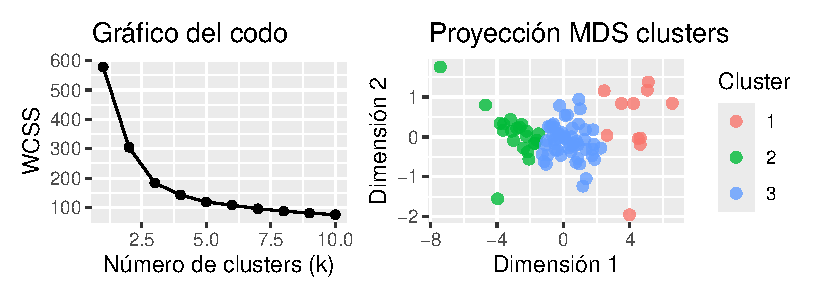
\includegraphics{ProyectoAED2024_files/figure-latex/unnamed-chunk-45-1} 

}

\caption{Gráfico del método del codo y representación mediante una proyección MDS de los clusters de k-means, con el parámetro $k$ escogido.}\label{fig:unnamed-chunk-45}
\end{figure}

El método del codo ilustrado en la Figura 13 parece indicarnos que la
mejor selección es \(k=3\) y observamos que los resultados parecen
satisfactorios. Por lo tanto, debido a la simplicidad del modelo nos
quedamos con esta elección. Pasamos a estudiar por separado el
comportamiento de cada clúster y trataremos de averiguar si tienen una
interpretación natural clara.

\begin{figure}

{\centering 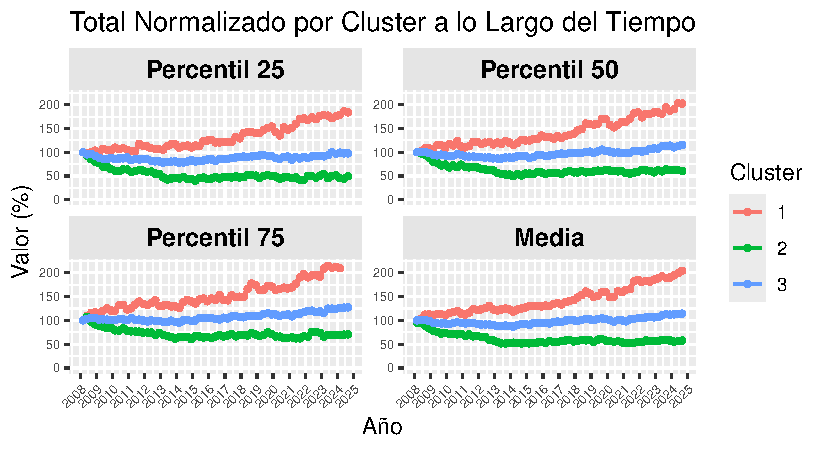
\includegraphics{ProyectoAED2024_files/figure-latex/unnamed-chunk-46-1} 

}

\caption{Evolución de los percentiles 25, 50, 75 y media de la evolución normalizada agrupados por clúster.}\label{fig:unnamed-chunk-46}
\end{figure}

Analizando los cuantiles y medias de cada clúster presentes en la Figura
14, se observa que se agrupan según rendimiento, cosa ya esperada
proviniendo de la métrica definida. Se observa que la mayoría de las
ramas de actividad se acumulan en los clústeres con la evolución
negativa o mediocre, en los cuales ha habido un decrecimiento (clúster
2) o estancamiento (clúster 3) de los trabajadores. Por otra parte el
clúster 1 parece presentar ramas con resultados positivos, aunque con
menor número de ramas que los anteriores.

Podemos observar que aquellos sectores relacionados con la
descontaminación o la programación y la informática han avanzado mucho
en los últimos años, mientras que los sectores más relacionados con la
construcción han caido fuertemente. Sin embargo, la conclusión general
es que la evolución del empleo en España durante los últimos años ha
sido marcadamente negativa para la mayoría de las ramas de actividad,
salvándose de ella ejemplos muy concretos. \newpage

%%%%%%%%%%%%%%%%%%%%%%%%%%%%%%%%%%%%%%%%%%

\vspace{6pt}

%%%%%%%%%%%%%%%%%%%%%%%%%%%%%%%%%%%%%%%%%%
%% optional

% Only for the journal Methods and Protocols:
% If you wish to submit a video article, please do so with any other supplementary material.
% \supplementary{The following supporting information can be downloaded at: \linksupplementary{s1}, Figure S1: title; Table S1: title; Video S1: title. A supporting video article is available at doi: link.}

%%%%%%%%%%%%%%%%%%%%%%%%%%%%%%%%%%%%%%%%%%







%%%%%%%%%%%%%%%%%%%%%%%%%%%%%%%%%%%%%%%%%%
%% Optional

%% Only for journal Encyclopedia


%%%%%%%%%%%%%%%%%%%%%%%%%%%%%%%%%%%%%%%%%%
%% Optional
\input{"appendix.tex"}
%%%%%%%%%%%%%%%%%%%%%%%%%%%%%%%%%%%%%%%%%%
\begin{adjustwidth}{-\extralength}{0cm}

%\printendnotes[custom] % Un-comment to print a list of endnotes


\reftitle{References}
\bibliography{mybibfile.bib}

% If authors have biography, please use the format below
%\section*{Short Biography of Authors}
%\bio
%{\raisebox{-0.35cm}{\includegraphics[width=3.5cm,height=5.3cm,clip,keepaspectratio]{Definitions/author1.pdf}}}
%{\textbf{Firstname Lastname} Biography of first author}
%
%\bio
%{\raisebox{-0.35cm}{\includegraphics[width=3.5cm,height=5.3cm,clip,keepaspectratio]{Definitions/author2.jpg}}}
%{\textbf{Firstname Lastname} Biography of second author}

%%%%%%%%%%%%%%%%%%%%%%%%%%%%%%%%%%%%%%%%%%
%% for journal Sci
%\reviewreports{\\
%Reviewer 1 comments and authors’ response\\
%Reviewer 2 comments and authors’ response\\
%Reviewer 3 comments and authors’ response
%}
%%%%%%%%%%%%%%%%%%%%%%%%%%%%%%%%%%%%%%%%%%
\PublishersNote{}
\end{adjustwidth}


\end{document}
